
\section{Examples}\label{sec:examples}

% 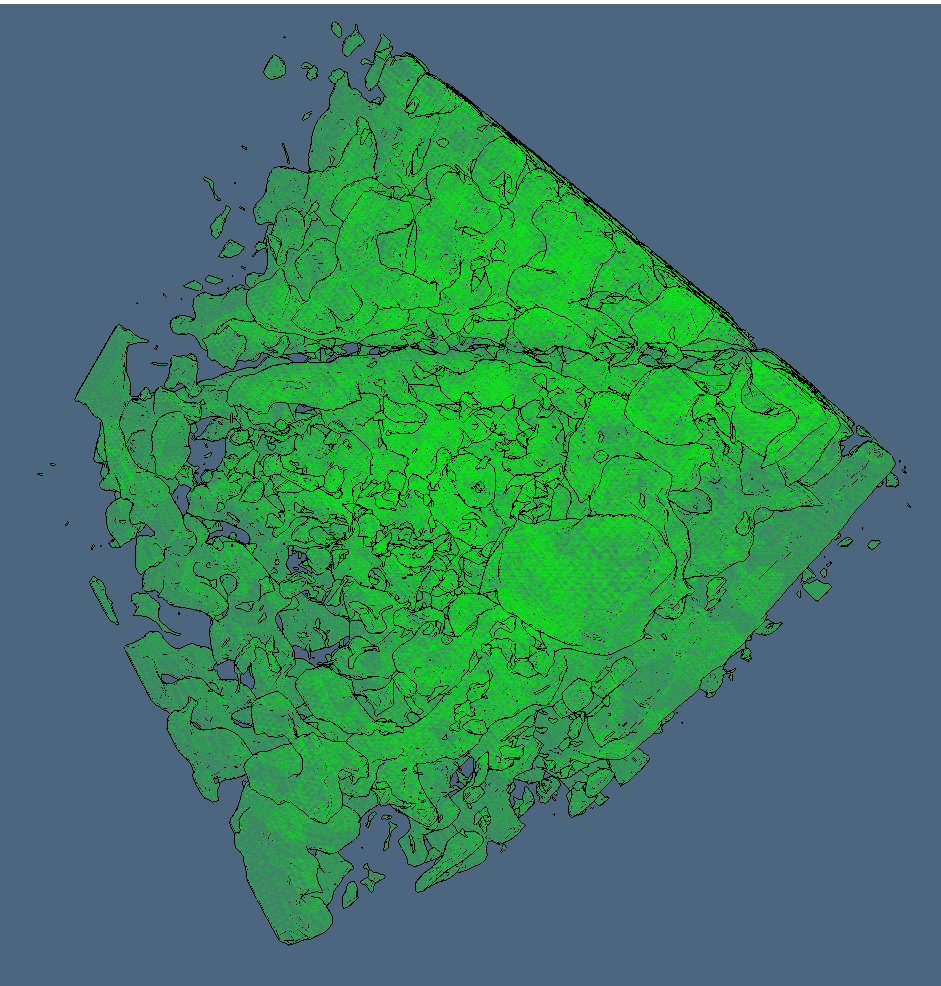
\includegraphics[height=0.3\textwidth]{figs/nrn10_100_green.png} 
%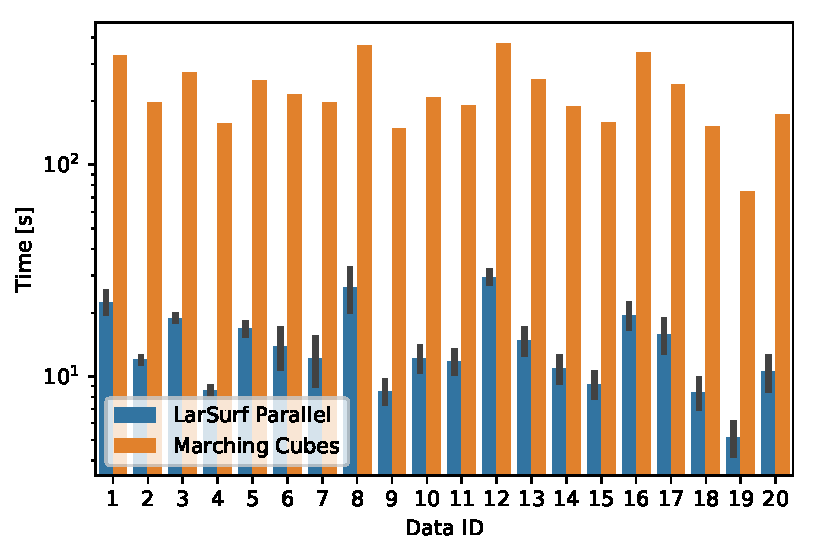
\includegraphics[scale=1]{input/ircad_comparison.pdf} 
\begin{figure}
\centering
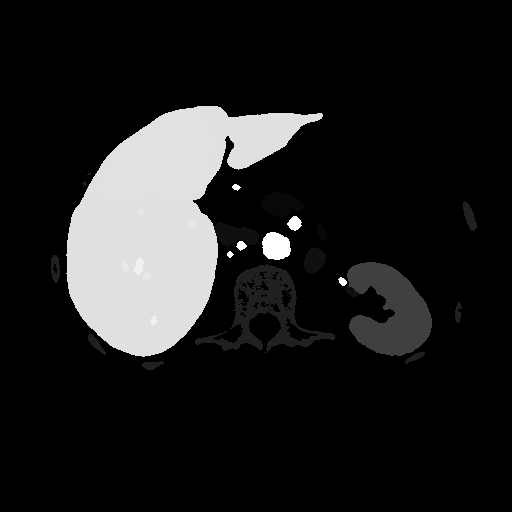
\includegraphics[width=0.40\textwidth]{src/figs/ircad01_segmentation_65.png}
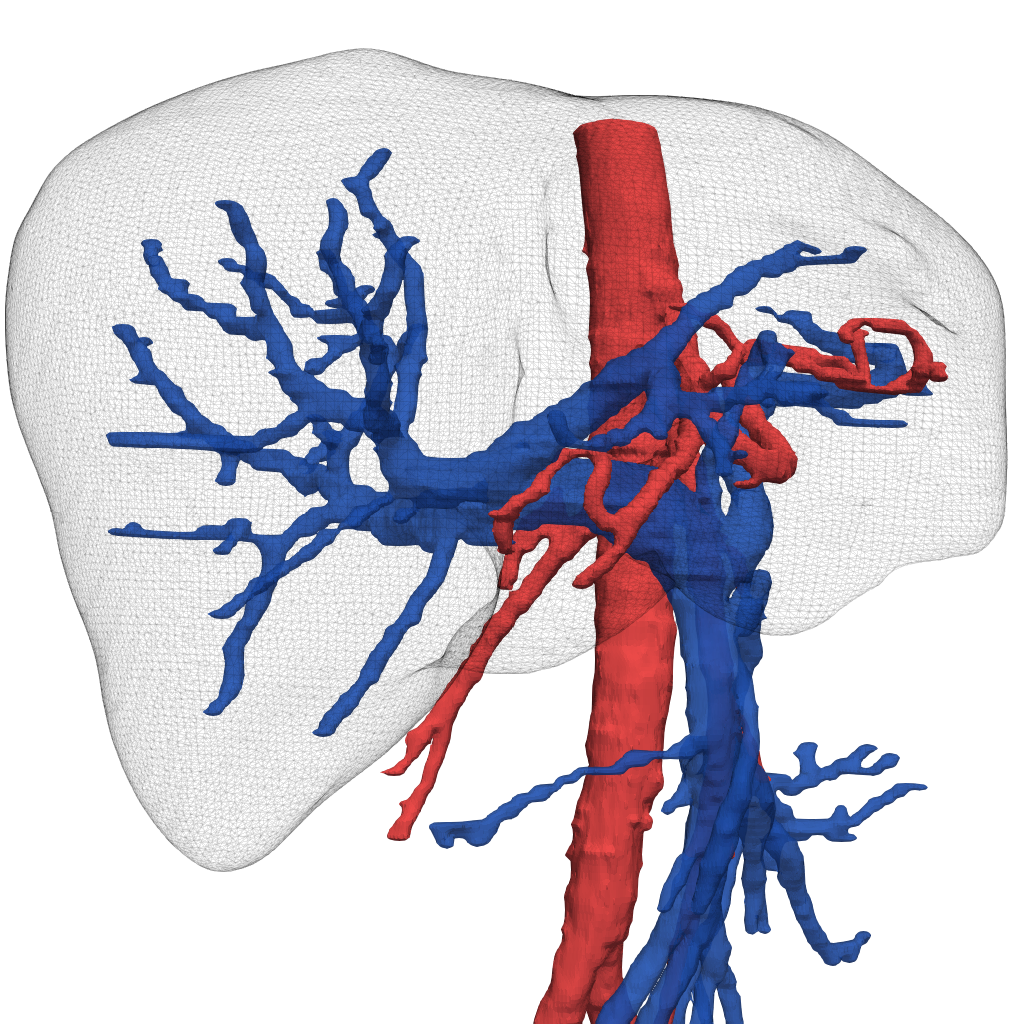
\includegraphics[width=0.40\textwidth]{src/figs/ircad01_liver_tricolore_01.png}
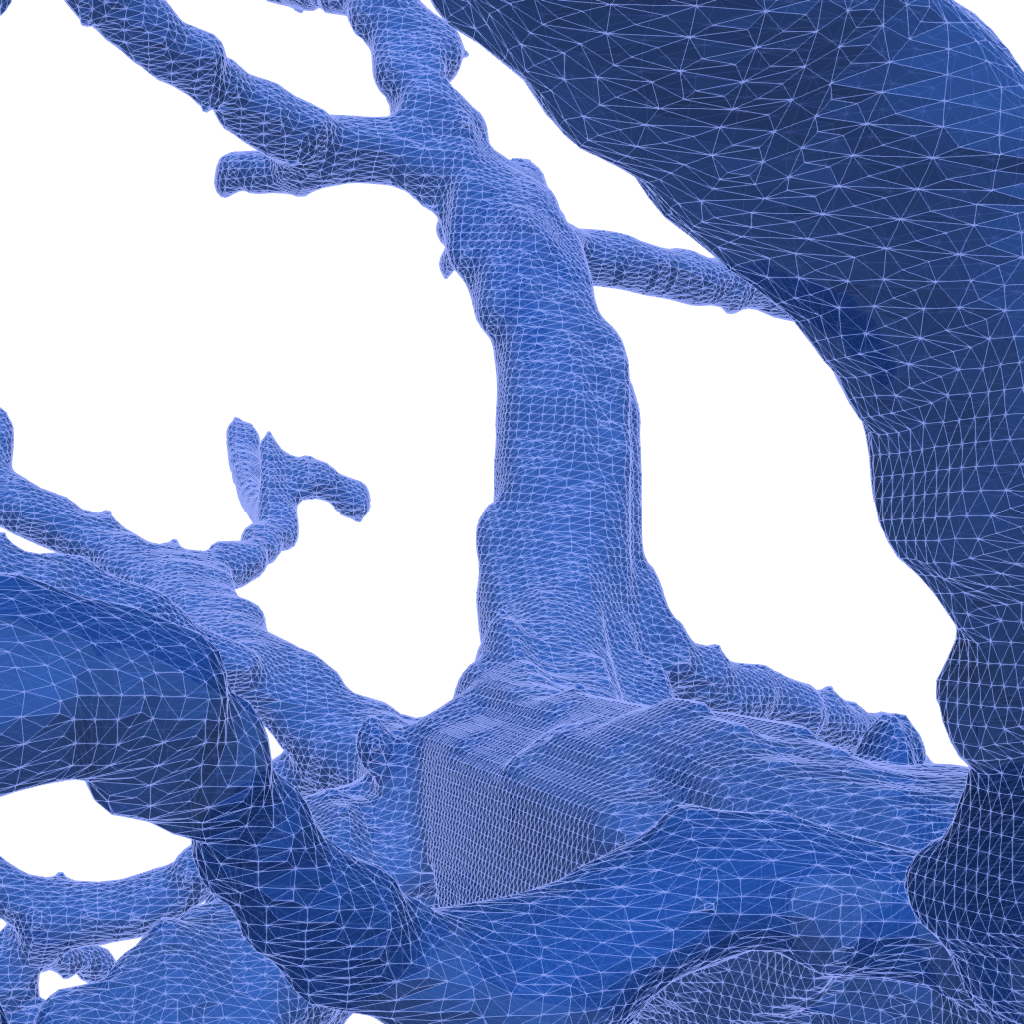
\includegraphics[width=0.40\textwidth]{src/figs/ircad01_porta_blue_01.png}
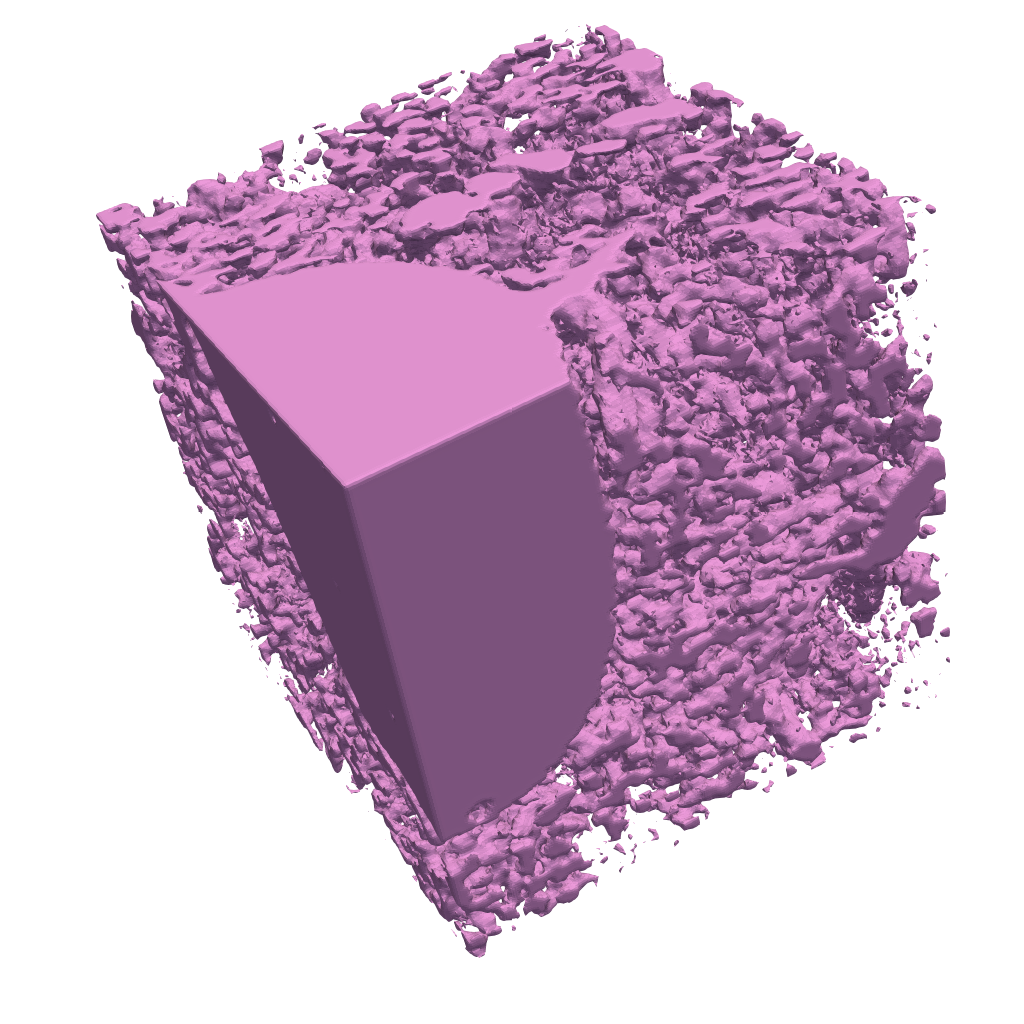
\includegraphics[width=0.40\textwidth]{src/figs/nrn10_200_pink_02.png}
% 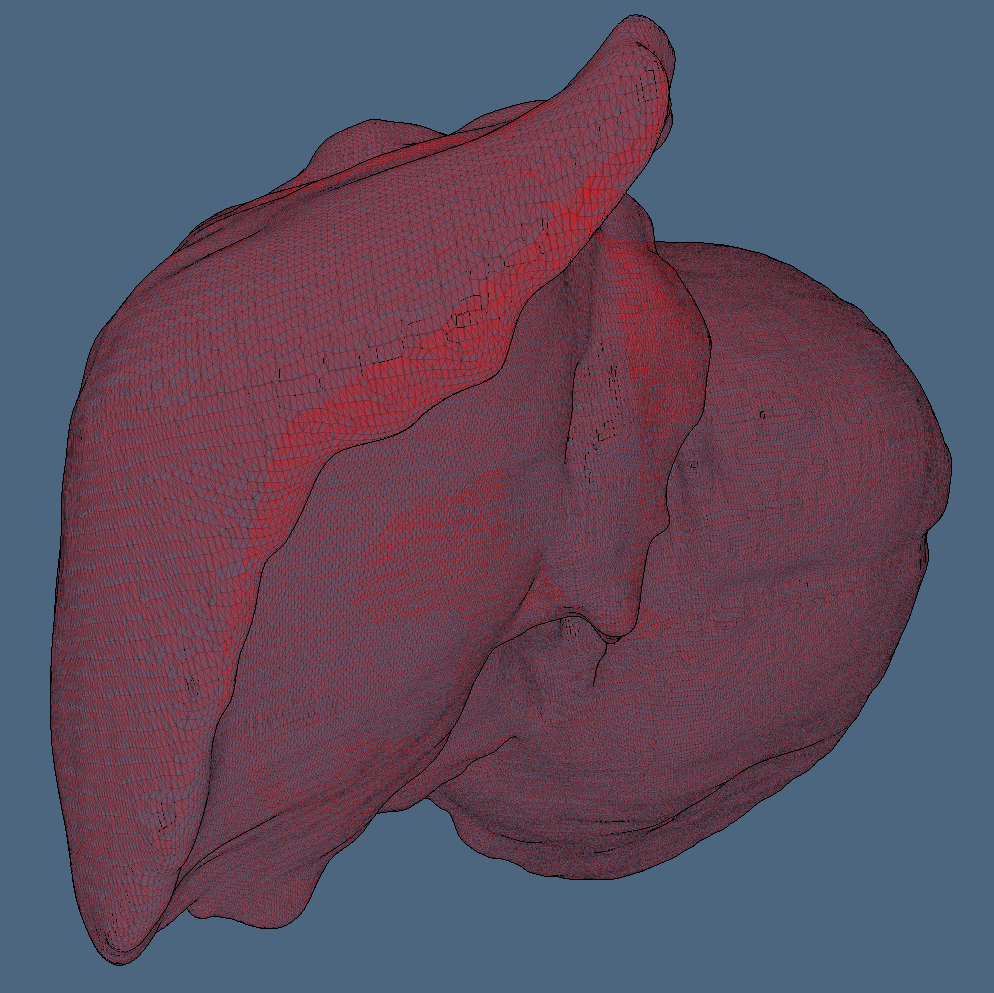
\includegraphics[width=0.4\textwidth]{figs/liver_01_red_3.png} 
% % \vspace{0.05\textwidth}
% 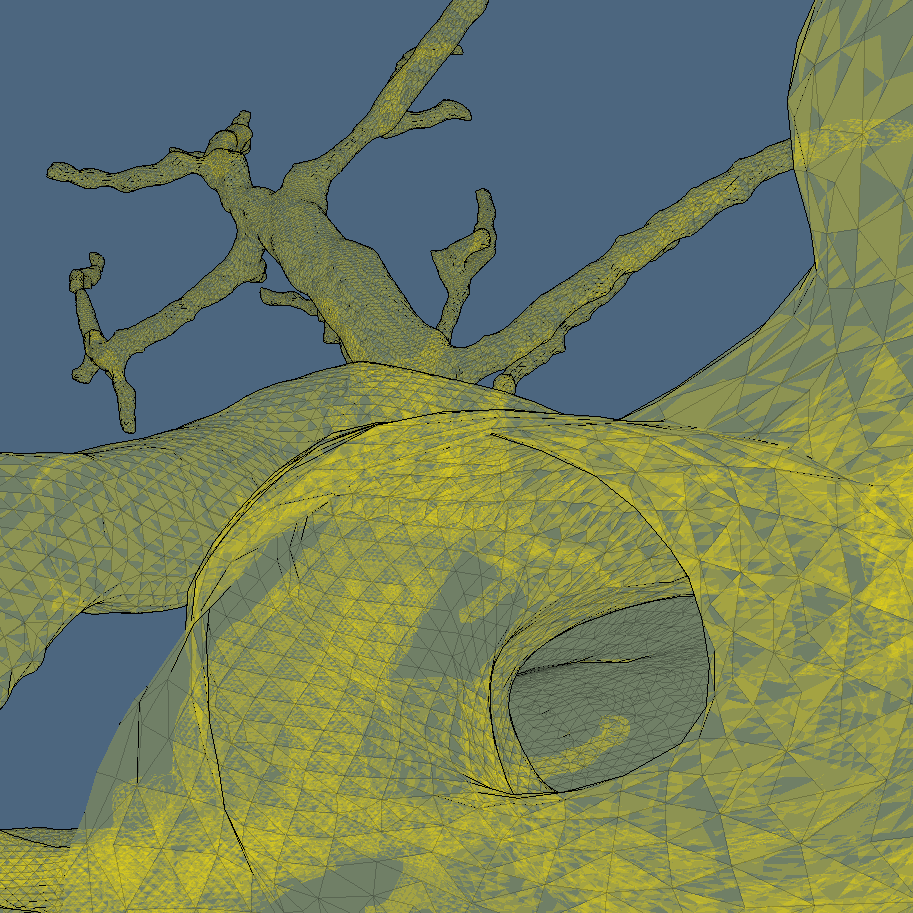
\includegraphics[width=0.4\textwidth]{figs/portalvein_01_yellow_3.png} 
% % \vspace{0.01\textwidth}
% 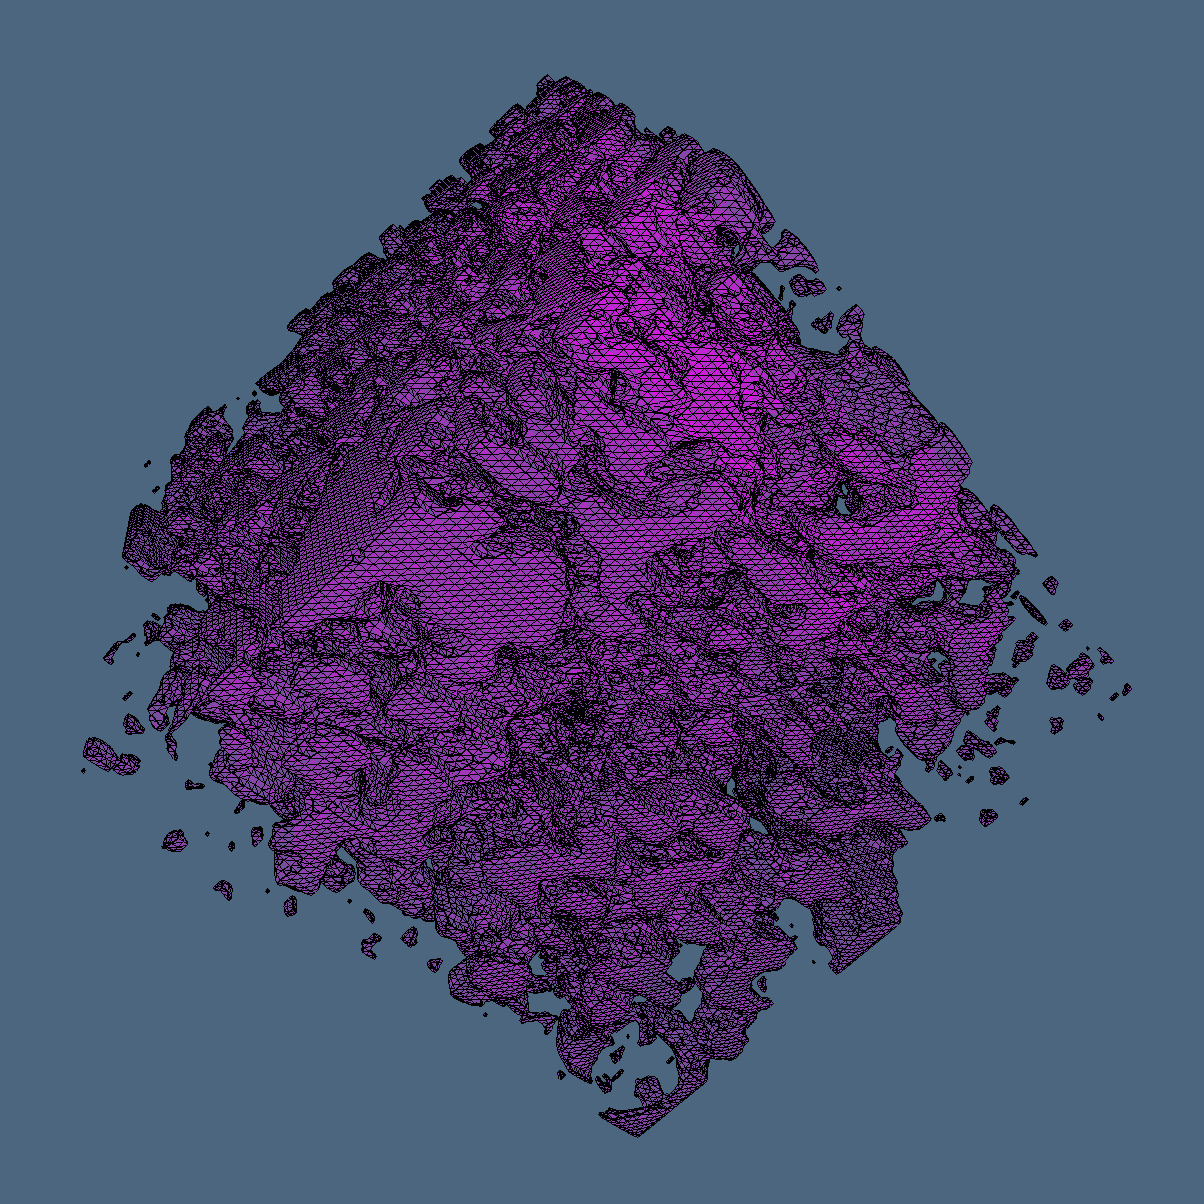
\includegraphics[height=0.4\textwidth]{src/figs/nrn10_100_magenta_high_res.png} 
% % 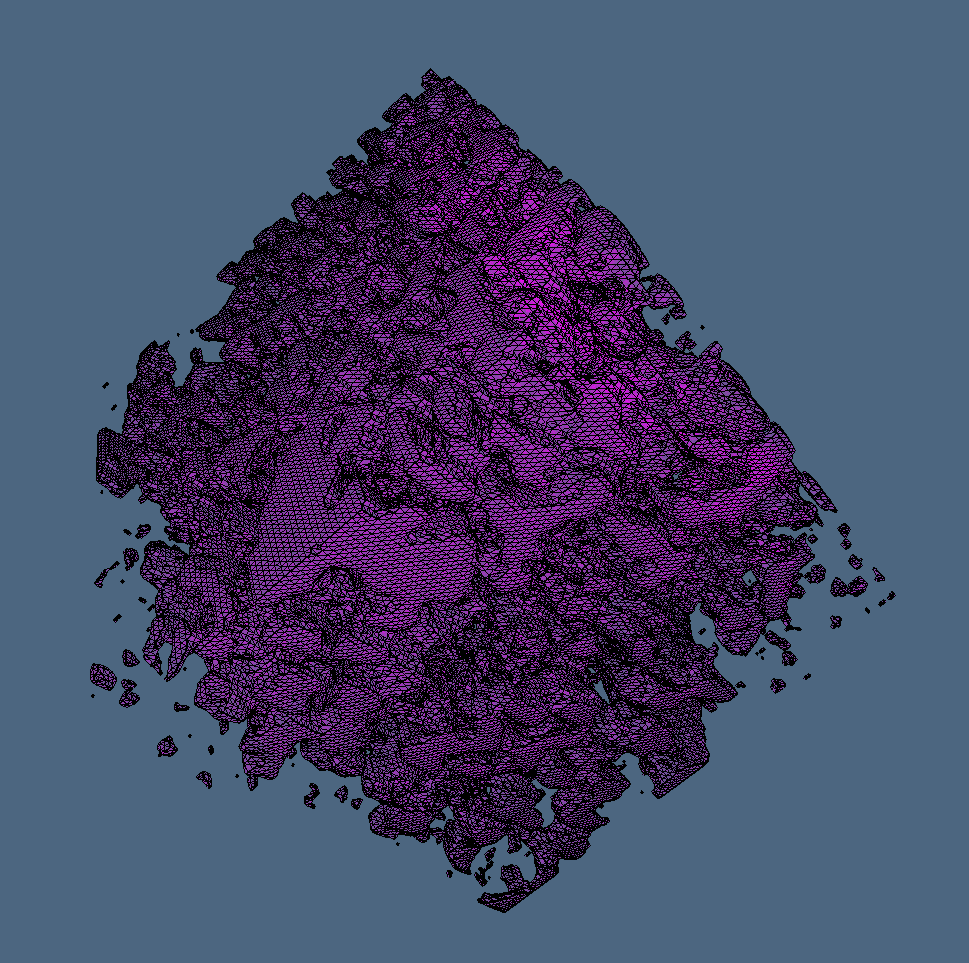
\includegraphics[height=0.4\textwidth]{figs/nrn10_100_low_res.png} 
% % \vspace{0.05\textwidth}
% 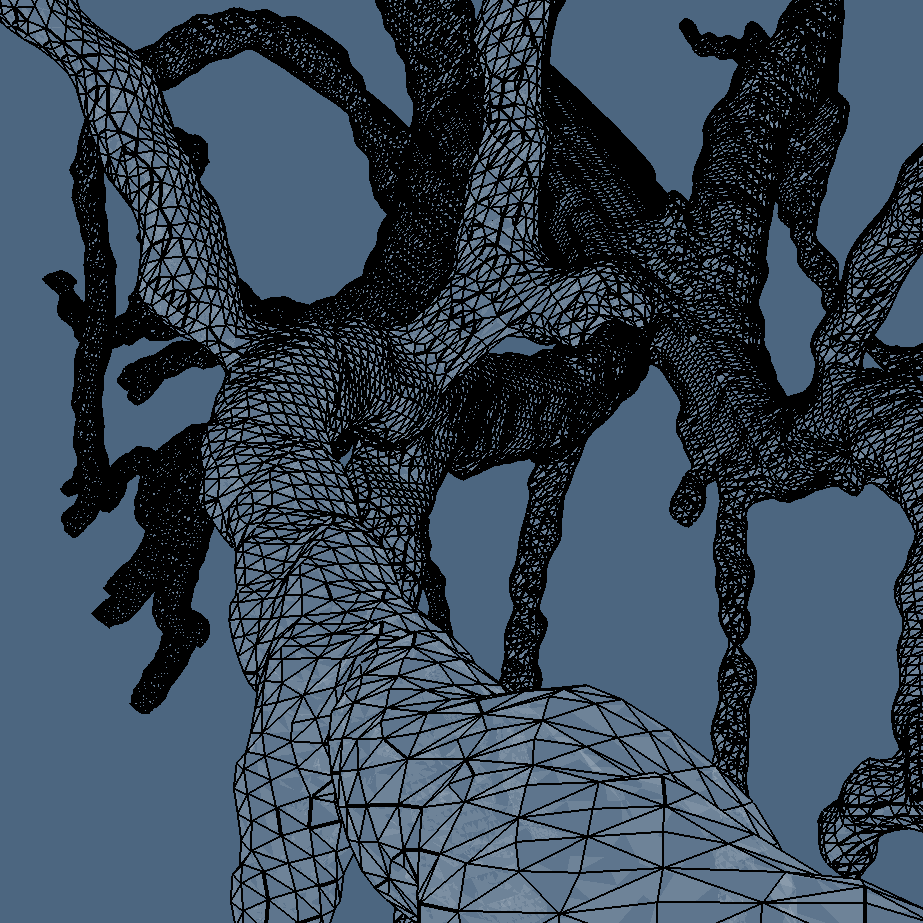
\includegraphics[width=0.4\textwidth]{figs/porta_smoothing_2.png} 
\caption{
Liver structures. The upper left image shows one slice  with segmented organs from  the Ircad dataset \cite{ircadb}.
The other images show the triangulated isosurfaces of the macroscopic and microscopic structures of the liver extracted with \textsc{lar-surf} algorithm. 
The wireframe model of the human liver along with the portal vein and hepatic artery can be seen on the upper right image. 
The left bottom image shows the detail of the portal vein  
with resolution $1.6\times0.57\times0.57$ $[mm]$.
On the bottom right image is shown the microvasculature of a pig liver based on corrosion cast prepared by Eberlova
\cite{eberlova2017use}. The size of the specimen is 0.936 $[mm]$ along each axis and the resolution of the Micro-CT data is 4.682 $\mu{}m$.
} \label{fig:example_liver_macro_micro}
\end{figure}
% Both right images show the Portal Vein from the same Ircad dataset \cite{ircad} 

% \begin{figure}
% \centering
% 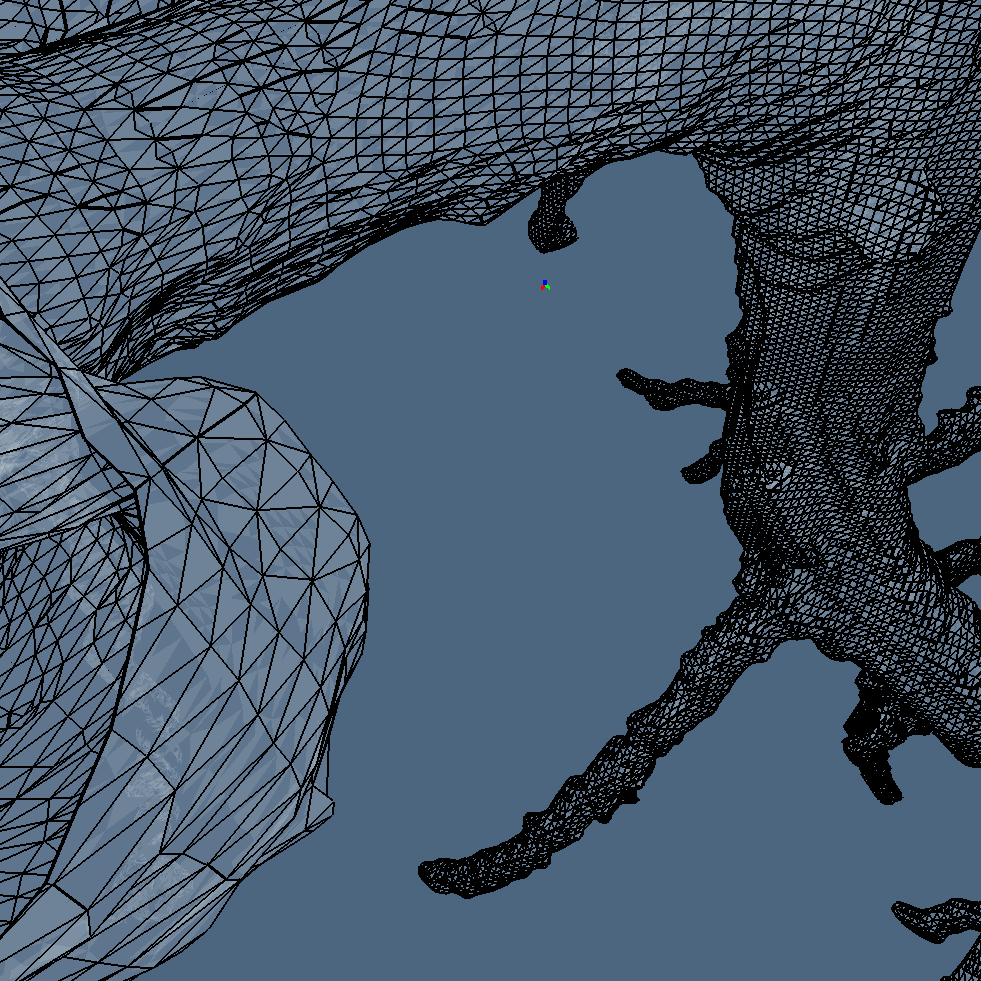
\includegraphics[width=0.4\textwidth]{figs/porta_smoothing_1.png} 
% \vspace{0.05\textwidth}
% 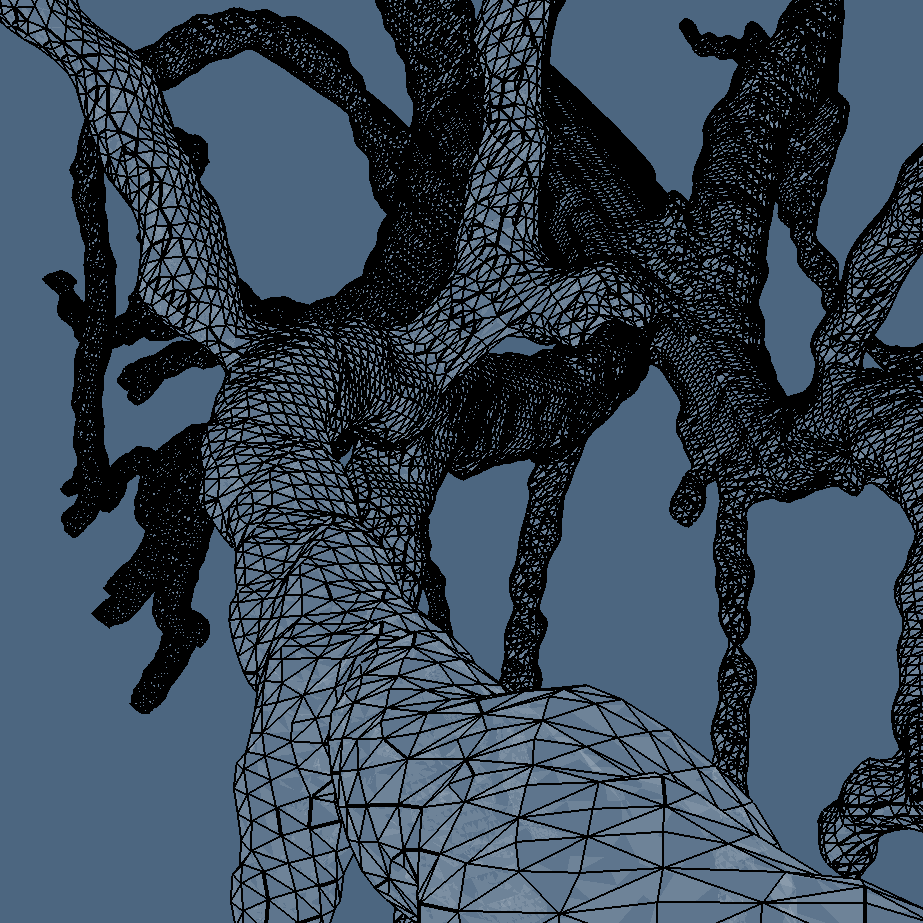
\includegraphics[width=0.4\textwidth]{figs/porta_smoothing_2.png} 
% %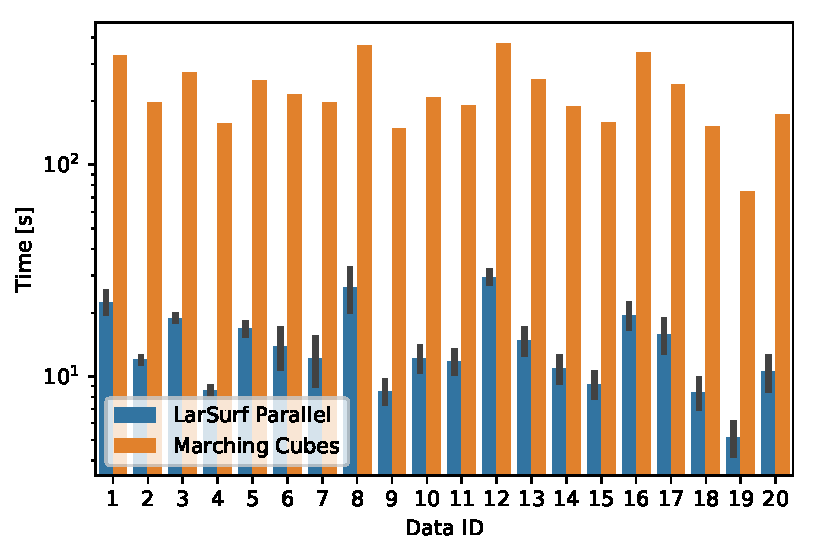
\includegraphics[scale=1]{input/ircad_comparison.pdf} 
% \caption{Triangulated isosurface of portal vein calculated with LAR-SURF}
% \label{fig:example_porta}
% \end{figure}

% The implementation of our algorithm is available in LarSurf package. 
Use of the \texttt{LarSurf.jl} package can be seen on listings \ref{lst:example1} where the liver segmentation with 2865131 voxels from the
Ircad dataset is used as an input for our surface extraction algorithm. The size of 3D volumetric 
image is $129 \times 512 \times 512$
and the voxel resolution is $1.6\times0.57\times0.57$ [mm]. 
The output liver surface model is formed by  182124 triangles and the number of vertices is 90822. 
The visualization can 
be seen in Fig. \ref{fig:example_liver_macro_micro}. 


\begin{lstlisting}[caption={Get surface from DICOM volumetric data}, label={lst:example1}]
using Distributed
using Pio3d  # Read 3D data from DICOM files
addprocs(3)  # set number of processors
using LarSurf

LarSurf.lsp_setup([64, 64, 64])  # set block size

# read data from DICOM files
datap = Pio3d.read3d("3Dircadb1.1/MASKS_DICOM/liver")
segmentation = datap["data3d"]
voxelsize_mm = datap["voxelsize_mm"]

# get surface
V, FV = LarSurf.lsp_get_surface(segmentation, voxelsize_mm)
FVtri = LarSurf.triangulate_quads(FV)

# do smoothing and save data
Vs = LarSurf.Smoothing.smoothing_FV_taubin(V,FV,0.5,-0.2,40)
objlines = LarSurf.Lar.lar2obj(Vs, FVtri, "liver.obj")
\end{lstlisting}

The portal vein surface extraction can be performed with a small change of input path in code.
The 3D image resolution is the same. 
% It can be seen in the same figure. 
The number of input voxels is 103533. 
The output surface is created by 90822 vertices and 182124 triangles. 

The right bottom image of Fig. \ref{fig:example_liver_macro_micro} is the surface of the microvasculature of pig liver. 
The volumetric image is based on Micro-CT data of corrosion casts of pig liver.
\cite{eberlova2017use}.
The size of the visualized data is $100\times100\times100$ voxels and the size of the voxel is 4.682 $\mu{}m$.
The number of triangles is 
544784 and the number of vertices is 272826.

% \begin{minted}{python}



% using Pkg
% \end{minted}
% \begin{minted}[breaklines,escapeinside=||,mathescape=true, linenos, numbersep=3pt, gobble=2, frame=lines, fontsize=\small, framesep=2mm]{julia}
% Your awesome julia code here\end{minted}




